\chapter{Theoretical Motivation}

\section{Nuclear Shell Model}
\label{sec:shell}
One of the greatest achievements of nuclear physics was the development of the nuclear shell model by \citet{Goeppert-Mayer_1950} and Jensen \textit{et al.}~\cite{Haxel_1949} which ultimately earned them the Nobel Prize in 1963.  In analogy to the noble gases (Group 18) in chemistry, certain configuration of protons and neutrons are more stable than others, suggesting the presence of ``magic numbers.''  Based on empirical data, it was apparent that nuclides comprised of 2, 8, 20, 28, 50, 82, or 126 protons or neutrons are particularly stable.  This stability must arise from the nature of the nuclear potential.  The presence of the magic numbers 2, 8, and 20 suggested that the nuclear potential must have a shape somewhere in between that of a harmonic oscillator and a square well.  Fig.~\ref{magic_numbers} shows that both of these potentials are able to reproduce the first three magic numbers.  However, neither potential succeeds in predicting the positions of the larger magic numbers.  Therefore, the simplified description of the nuclear potential must be missing something.

\begin{figure}%
\centering
\fbox{

\includegraphics[width=\columnwidth,height=0.9\textheight,keepaspectratio]{numbers}%
%}
%\fbox{
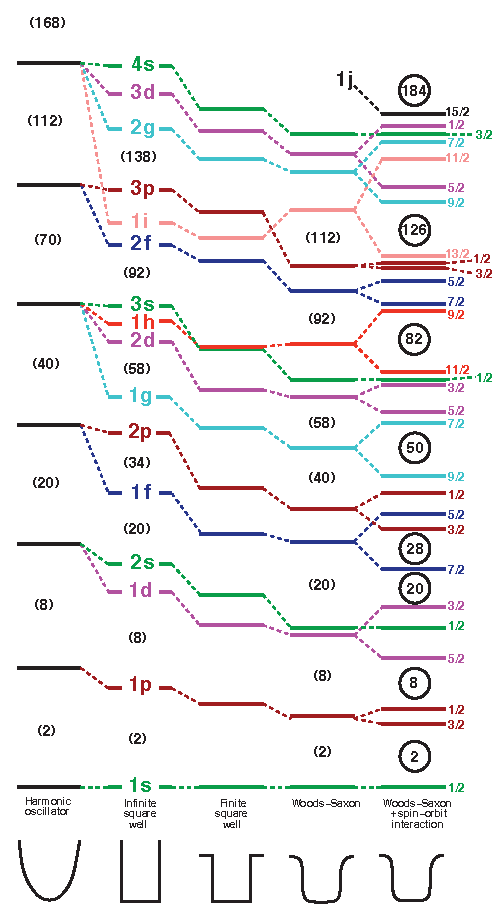
\includegraphics[width=\columnwidth,height=0.9\textheight,keepaspectratio]{Kay_Thesis_23}%
}
\caption[Nuclear energy levels based on different potentials leading to the magic numbers]{Nuclear energy levels based on different potentials leading to the magic numbers.  The oscillator number is given at left.  Numbers in parentheses are the magic numbers predicted using the specified potential.  The circled numbers in the right column corresponding to the Woods-Saxon potential with a spin-orbit interaction are the nuclear magic numbers close to stability.  Figure modified from Ref.~\cite{Kay_2007}.}%
\label{magic_numbers}%
\end{figure}

The shape of a potential that is between that of a harmonic oscillator and a square well is the Woods-Saxon potential
\begin{equation}
f(r,r_0,a)=\left[1+\exp \left(\frac{r-r_0}{a}\right)\right]^{-1} \qquad \textrm{Woods-Saxon}
\label{eq:woods_saxon}
\end{equation}
where $r$ is the dependent variable (the radius), $r_0=RA^{1/3}$ is the nuclear radius; $R$ has a typical value of 1.25\,fm and $a$, the diffuseness parameter, is on the order of 1\,fm. 
The fundamental shape of this potential is shown in Fig.~\ref{magic_numbers}; a function plot of this potential is given in Fig.~\ref{potentials}.  The degeneracy of each level produced by the Woods-Saxon potential and the square well, both central potentials, is $2(2\ell+1)$, where $\ell$ is the orbital angular momentum of the state.  Although the Woods-Saxon potential shifts the position of the energy levels relative to the finite square well, it still does not reproduce the magic numbers observed in experiment.

\begin{figure}%
\centering
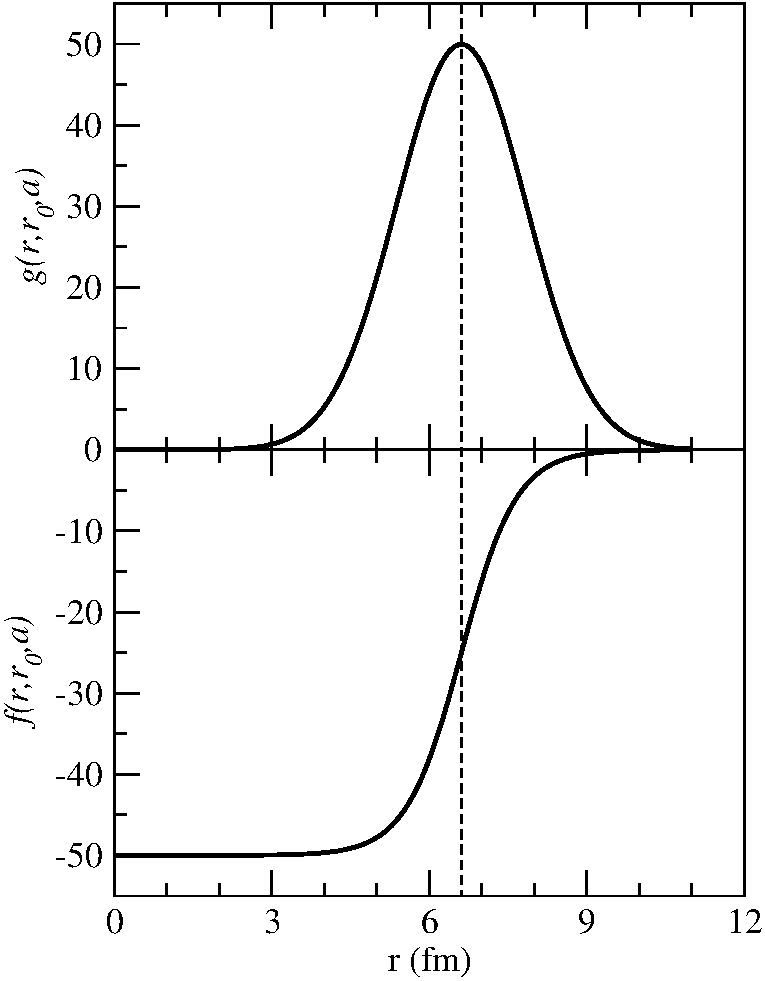
\includegraphics[width=\columnwidth,height=0.33\textheight,keepaspectratio]{potentials}%
\caption[Functional plot of the Woods-Saxon potential]{Functional plot of the Woods-Saxon potential.  The volume potential $f(r)$ (Eq.~\ref{eq:woods_saxon}) and the surface-derivative potential $g(r)$ (Eq.~\ref{eq:surface}) are plotted.  The depth of the well has been selected to be 50\,MeV.  The dashed line indicates the nuclear radius $R=6.6$\,fm, corresponding to an $A=28$ nucleus.}%
\label{potentials}%
\end{figure}

The breakthrough of Goeppert-Mayer and Jensen \textit{et al.} is the inclusion of the non-central nuclear spin-orbit potential.  %At the time, 
The idea of spin-orbit coupling was already well-known in chemistry, arising from the electromagnetic interaction between a nucleus and an orbiting electron.
  The general form of the nuclear spin-orbit potential is the same as the atomic spin-orbit potential.  However, empirically, the nuclear spin-orbit potential arises from the nucleon-nucleon interaction is of opposite sign and 20--30 times stronger than atomic spin orbit potential~\cite{Krane_1988,Satchler_1990}.  The nuclear potential is then rewritten as 
\begin{equation}
U(r)=-V f(r,R,a)+V_\mathrm{SO} \frac{1}{r} \frac{d}{dr} f(r,R,a) (\vec{\ell}\cdot\vec{s}) 
\qquad \textrm{Thomas form}
\label{eq:optical}
\end{equation}
where $V$ and $V_\mathrm{SO}$ are the depth of the volume and surface-peaked potentials, respectively. 
 The depth of the volume potential $V$ is typically on the order of 50\,MeV.  With this new potential, each level with $\ell>0$ is split into two new levels.  For a given value of $\ell$, the $j=\ell+\frac{1}{2}$ state has lower energy, and the $j=\ell-\frac{1}{2}$ state has higher energy.  The energy difference is proportional to $\frac{1}{2}(2\ell+1)\hbar^2$.  Starting with the $n=3$ oscillator shell (2$p$1$f$), the highest angular momentum state is pushed down to energies comparable to the preceding oscillator shell (see Fig.~\ref{magic_numbers}). This is the interaction which correctly reproduces the observed magic numbers 28--126.

The stable nuclei with closed proton and neutron shells, such as $^{40}$Ca and $^{208}$Pb, have been well understood within the context of the shell model for decades.  However, only recently has it been possible to study experimentally  exotic nuclei around the neutron-rich double shell closure of $Z=50$, $N=82$.  As such, the doubly-magic $^{132}$Sn nucleus is the subject of increasing attention in the nuclear physics community.  With the development of the Helical Orbit Spectrometer (HELIOS) and the Californium Rare Isotope Breeder Upgrade (CARIBU) at the ATLAS facility of Argonne National Laboratory, ground-breaking measurement opportunities are on the horizon.

\section{The Stellar \textit{r}-process}
\label{astro}
\subsection{Background}
In 1957, the seminal work ``Synthesis of the Elements in Stars'' by Burbidge, Burbidge, Fowler, and Hoyle laid the foundation of understanding nucleosynthesis in the universe~\cite{Burbidge_1957}.  An important process in stellar nucleosynthesis is the rapid neutron capture process ($r$-process), which accounts for synthesis of about half of the chemical elements with atomic mass greater than $A=50$~\cite{Martinez-Pinedo_1999}.  
Nuclei involved in the stellar $r$-process are therefore of key importance in understanding the isotropic abundances found in the universe.  The $r$-process occurs in environments of extreme neutron flux, where free neutron density is on the order of $n_n\geq10^{21}$\,cm$^{-3}$, and temperatures in the $T\geq1$\,GK range~\cite{Iliadis_2007}.  

Based on these extreme environmental parameters, a number of exotic sites of the $r$-\-pro\-cess have been suggested~\cite{Surman_2009}, however a likely candidate is the stellar atmosphere during a core-collapse supernova, leading to the creation of a neutron star.  In such an environment, nuclei capture an increasing number of neutrons creating more and more neutron-rich isotopes.  When the environmental temperatures decrease, reducing the rate of neutron capture, $\beta$-decay becomes dominant.  The neutron-rich isotopes typically $\beta$-decay along a path of constant $A$ back towards stability. The transition from the neutron capture  regime to the $\beta$-decay regime is called \textit{freeze-out}.

One of the major influencing factors that dictates the path of the $r$-process is the competition between neutron capture ($n$,$\gamma$) and photodisintegration ($\gamma$,$n$).  As a nucleus captures successive neutrons, each added neutron has a lower binding energy.  This process continues until the neutron capture rate $\lambda_n$ is balanced by the photodisintegration rate $\lambda_\gamma$.  When the two reactions are in thermal equilibrium, $(n,\gamma)\leftrightharpoons(\gamma,n)$, and can be described by Maxwell-Boltzmann statistics, the isotopic abundance is determined by the Saha equation%, shown in Eq.~\ref{eq:saha}. 

\begin{equation}
\begin{split}
\frac{n(Z,A+1)}{n(Z,A)}&=n_n \left(\frac{2\pi \hbar^2}{m_nkT}\right)^{3/2} \frac{(2j_{Z,A+1}+1)}{(2j_{Z,A}+1)(2j_n+1)}\frac{G^\mathrm{norm}_{Z,A+1}}{G^\mathrm{norm}_{Z,A}}e^{Q_{n\gamma}/kT} \qquad \textrm{Saha equation}\\
& \propto n_n \left(\frac{2\pi \hbar^2}{m_nkT}\right)^{3/2} e^{Q_{n\gamma}/kT}\\
\end{split}
\label{eq:saha}
\end{equation}
where $n(Z,A)$ is the number density (abundance) of the nuclide $^A_ZX$, $k$ is the Boltzmann constant, $j_i$ and $G^\mathrm{norm}_{i}$ are the spins and normalized partition functions of the individual particles, respectively; and $Q_{n\gamma}$ is the neutron capture $Q$-value, or equivalently, the neutron separation energy $S_n$ of $^{A+1}_{~~~~Z}X$.
The second line of the equation is a simplification to illustrate that the abundance of adjacent isotopes depends largely on the neutron density $n_n$, the temperature $T$, and the ($n$,$\gamma$) neutron capture $Q$-value.
When the reaction rates are in equilibrium, in order for the rapid neutron capture to continue, the nucleus must undergo negative $\beta$-decay.  It is said during this time that the $r$-process is ``waiting'' for the $\beta$ decay; this assumption is called the \textit{waiting-point approximation}.

Nuclei along the $r$-process path with longer $\beta$-decay half-lives have a substantial effect on the $r$-process.  While the isotopic abundance is governed by the neutron capture $Q$-value, the elemental abundance is inversely proportional to the total $\beta$-decay rate of the isotopic chain (\textit{steady flow approximation})~\cite{Iliadis_2007}. In particular, the relatively more-stable nuclei with magic neutron numbers cause a pause in the $r$-process.  This pause leads to a greater abundance of these nuclide during the 
$r$-process, corresponding to greater solar abundance in the same mass region after $r$-process freeze-out.
These so-called ``waiting-point'' nuclei at $N=50$, 82, and 126 correspond to the three predominant peaks in the isotropic abundance spectrum shown in Fig.~\ref{abun} said to be produced by the $r$-process~\cite{Kratz_1993}.   The effect of these waiting points is so substantial that the time it takes for a seed nucleus to travel the $r$-process path is largely determined by the sum of the half-lives of nuclei near closed neutron shells~\cite{Martinez-Pinedo_1999}.  As a result, it is clear that knowledge of the shell gaps of exotic isotopes in the region of the magic numbers is essential to understanding stellar processes.  Specifically, energy levels of isotopes near the doubly-magic $^{132}$Sn shell closure are vital to understanding the synthesis of isotopes in the $A=130$ region (see Fig.~\ref{abun}).

\begin{figure}%
\centering
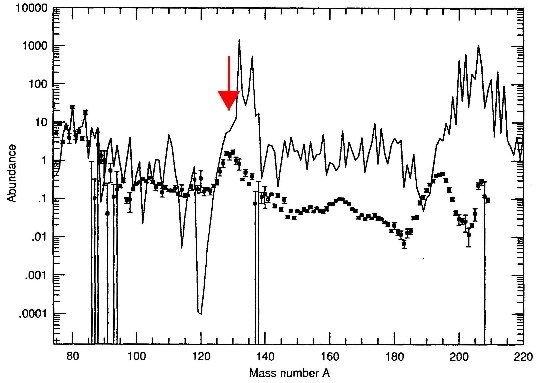
\includegraphics[width=\columnwidth,height=0.33\textheight,keepaspectratio]{Kratz_1993-fig62}%
\caption[Observed and calculated stellar $r$-process abundances]{Observed and calculated stellar $r$-process abundances.  The calculated isobaric abundances (curve) are based on the waiting-point and steady-flow approximations (described in the text) with $T_9=1.3$ and $n_n=10^{20}$\,cm$^{-3}$. Note peak near $A=130$ (indicated with arrow).  Annotated figure taken from Ref.~\cite[Fig.~6(a)]{Kratz_1993}.}%
\label{abun}%
\end{figure}

\subsection{Theoretical Framework}
Until recently, the only way to investigate the unstable neutron-rich nuclei of the $r$-process was through theoretical calculations.  The first shell-model calculations were performed in the late 1960s and early 1970 with the advent of powerful computing systems.  The following decades saw the development of advanced microscopic interaction models such as Skyrme and Gogny~\cite{Caurier_2005}.  As the development of facilities for radioactive beams drew nearer in the early 1990s, the shell properties of heavy neutron-rich isotopes gained renewed interest.  Many theorists sought to extrapolate models that described $\beta$-stable nuclei to exotic nuclei along the $r$-process path~\cite{Sharma_2002}.  An illustrative example is the comparison of predictions of mass models.  While the models tend to agree in the regions with experimental data, they diverge wildly when extrapolated to exotic nuclei as shown in Fig.~\ref{quench}~\cite{Dillmann_2003}.

\begin{figure}%
\centering
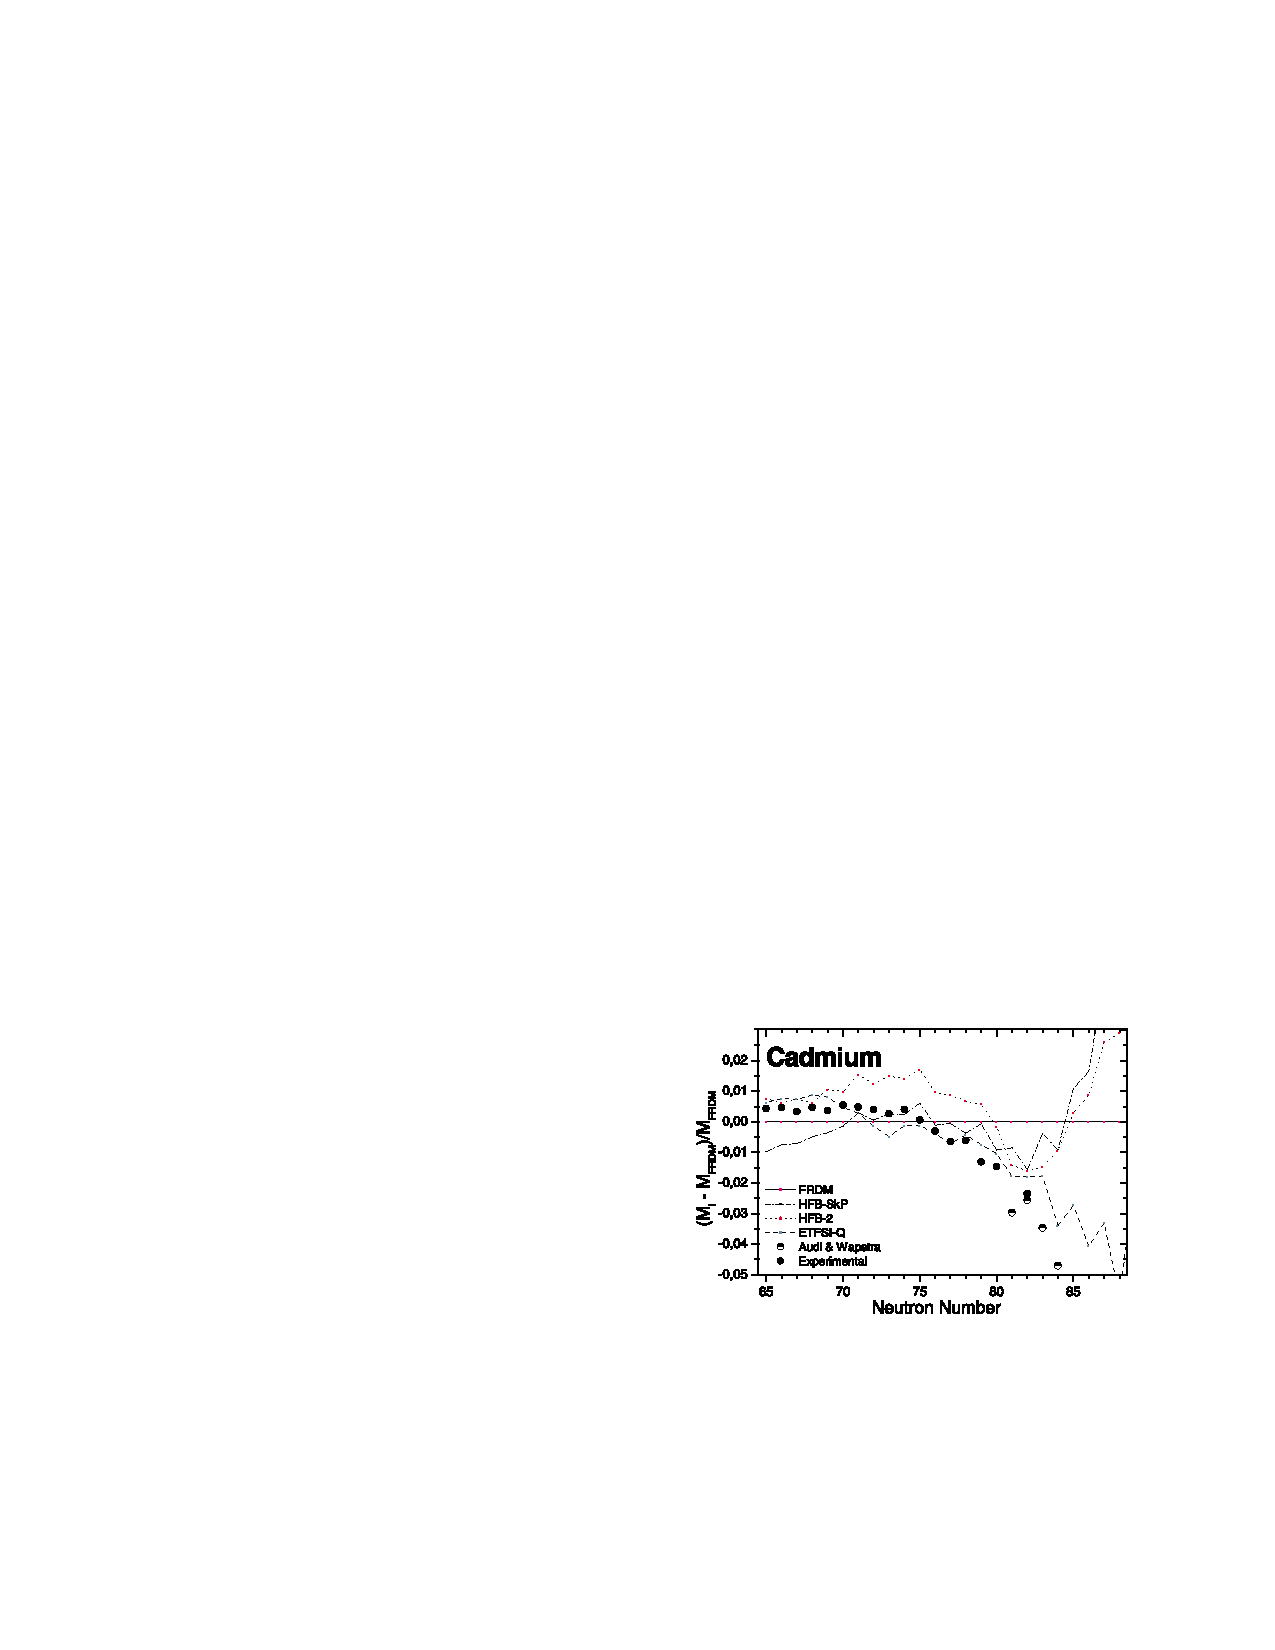
\includegraphics[width=0.75\columnwidth,keepaspectratio]{Dillmann_2003-fig3}%
\caption[Illustration of shell quenching in the Cd isotopes ($Z=48$)]{Illustration of shell quenching in the Cd isotopes ($Z=48$).  Measured isotope masses (full circles), short-range mass extrapolations (half-circles) and calculated masses (lines) are plotted relative to the finite-range liquid droplet model (FRDM).  Mass trends below the FRDM line are a signature of shell quenching.  Figure from Ref.~\cite[Fig.~3]{Dillmann_2003}}%
\label{quench}%
\end{figure}

The lack of a shell model that globally fits experimental results thus invited theorists to apply a variety of techniques to try to predict the evolution of nuclear structure with increasing neutron excess towards  the $r$-process nuclei (and beyond to the neutron drip line).  For example, the Hartree-Fock-Bogoliubov (HFB) calculations using the Skyrme force SkP and the relativistic mean-field (RMF) approximation both show significantly different predictions for properties of exotic nuclei than for $\beta$-stable nuclei.  While both models showed similar increased diffuseness in the neutron potential, they disagreed dramatically in their predictions of the spin-orbit splitting~\cite{Dobaczewski_1994}.

As discussed in \S\,\ref{sec:shell}, the effect of spin-orbit splitting is a fundamental factor influencing the formation of magic number shell gaps.   More specifically, it is the presence of a non-central spin-orbit term in the nuclear potential that produces the shell gaps in the naive shell model~\cite{Krane_1988}.   This effect is shown in the rightmost column of Fig.~\ref{magic_numbers}.  As shown in Eq.~\ref{eq:optical}, the spin-orbit potential, and thus the spin-orbit splitting, is proportional to the gradient of the nuclear potential~\cite{Grawe_2005}.  The diffuse nuclear surface and larger spacial extent of neutron-rich nuclei can produce a softening of the nuclear potential.  The resultant weakening of the spin-orbit potential reduces, or otherwise alters, the shell gaps~\cite{Schiffer_2004}.

Another important aspect of shell spacing is the effect of the tensor force, the effect of which is \textit{not} shown in Fig.~\ref{magic_numbers}.  The tensor component of the nuclear potential connects the $^3S_1$ ($L=0$) angular momentum state and the $^3D_1$-state ($L=2$) in the deuteron to produce the measured magnetic dipole and electric quadrupole moments~\cite{Wong_1998}.  In a similar fashion, the tensor force connects single-particle orbitals above closed nuclear shells.  The interaction between adjacent levels can be either attractive (deuteron-like) or repulsive and is responsible for trends in spacing of single particle levels~\cite{Otsuka_2005}.% (see Fig.~3).\marnote{figure referenced}

If the shell gaps diminish or are not present, the shell effects are said to be ``quenched.''  This was an early prediction of the HFB method and suggested that the $N=82$ shell closure may be quenched along the $r$-process path.   However, without making any assumptions about shell quenching in the model, the SkP force used in the HFB calculations intrinsically predicts smaller shell gaps than in other models~\cite{Sharma_2002}.  Furthermore, when applied to shell gaps for which experimental data exists, not only does SkP underestimate the shell gaps, it does not fit the data as well as other calculations, such as relativistic Hartree-Bogoliubov (RHB) model. 

That is not to say that shell quenching does not happen.  Any reasonable force model shows decreasing shell gaps, \textit{i.e.}, lower  as nuclei become more neutron-rich.  This reduction of the shell gaps is due to the decreasing neutron separation energy as more neutrons are added to the nucleus, which is a key feature of the $r$-process.  As the binding energy of each additional neutron becomes smaller and smaller, the shell gap eventually disappears.  With enough neutron excess, all of the shell gaps quench at the \textit{terminus stratum} of the neutron drip line.

\subsection{Initial Measurements}
In the absence of further experimental data, it would remain an open question where shell quenching occurred among the $N=82$ isotones and to what extent the effect was present in $^{132}$Sn.  In the meantime, the predictions from models explicitly involving shell quenching and experimental data from a suite of $\beta$-decay studies performed at the ISOLDE facility at CERN would seem to support a reduction of the shell gap above $N=82$.  The experimental evidence offered by the first of these studies was inconclusive due to isobaric contamination but suggested a relatively small $E$(2$^+$) value of 957\,keV for $^{130}$Cd~\cite{Kautzsch_2000}.  The follow-up study utilized significantly more advanced background suppression, but showed inconsistent results for cadmium and tin~\cite{Dillmann_2003}.  These studies emphasized the difficulties of these measurements and the need for further measurements while leaving the $N=82$ shell gap on uncertain ground.

More recently, two experiments have brought about a ``restoration'' of the $N=82$ shell gap in $^{132}$Sn.  The first was a study done at GSI that measured $\gamma$-ray transitions in $^{130}$Cd, which at the time of publication was the most neutron-rich $N=82$ isotope with observed  $\gamma$-ray transitions~\cite{Jungclaus_2007}.  The $^{130}$Cd isomers were produced in a knockout reaction and in a beam-fragmentation reaction.  What made this study unique is that it measured $\gamma$-ray transitions in coincidence with ions unambiguously identified using a fragment separator.  By measuring the transitions in coincidence with explicit ion identification, it was clear the $\gamma$-rays were being produced in isomeric decay of the isotone of interest.  The study measured a larger $E$(2$^+$) value than found in previous studies, strengthening the argument for the $N=82$ shell gap.  

Further reinforcement came from another experiment performed at CERN with ISOLDE.  This most recent study was a mass measurement using the ISOLTRAP Penning trap mass spectrometer~\cite{Dworschak_2008}.  In order to circumvent problems with isobaric contamination, the $^{132}$Sn was made into a sulfide and the resultant $^{132}$Sn$^{34}$S$^+$ was then separated and analyzed.  The subsequent mass measurement differed from the previously accepted value for $^{132}$Sn by 480\,keV.  This new mass value also increases the accepted value of the two-neutron separation energy $S_{2n}$ for $^{132}$Sn, giving it the largest shell gap of the $N=82$ isotones (see Fig.~\ref{50_gap}).

\begin{figure}%
\centering
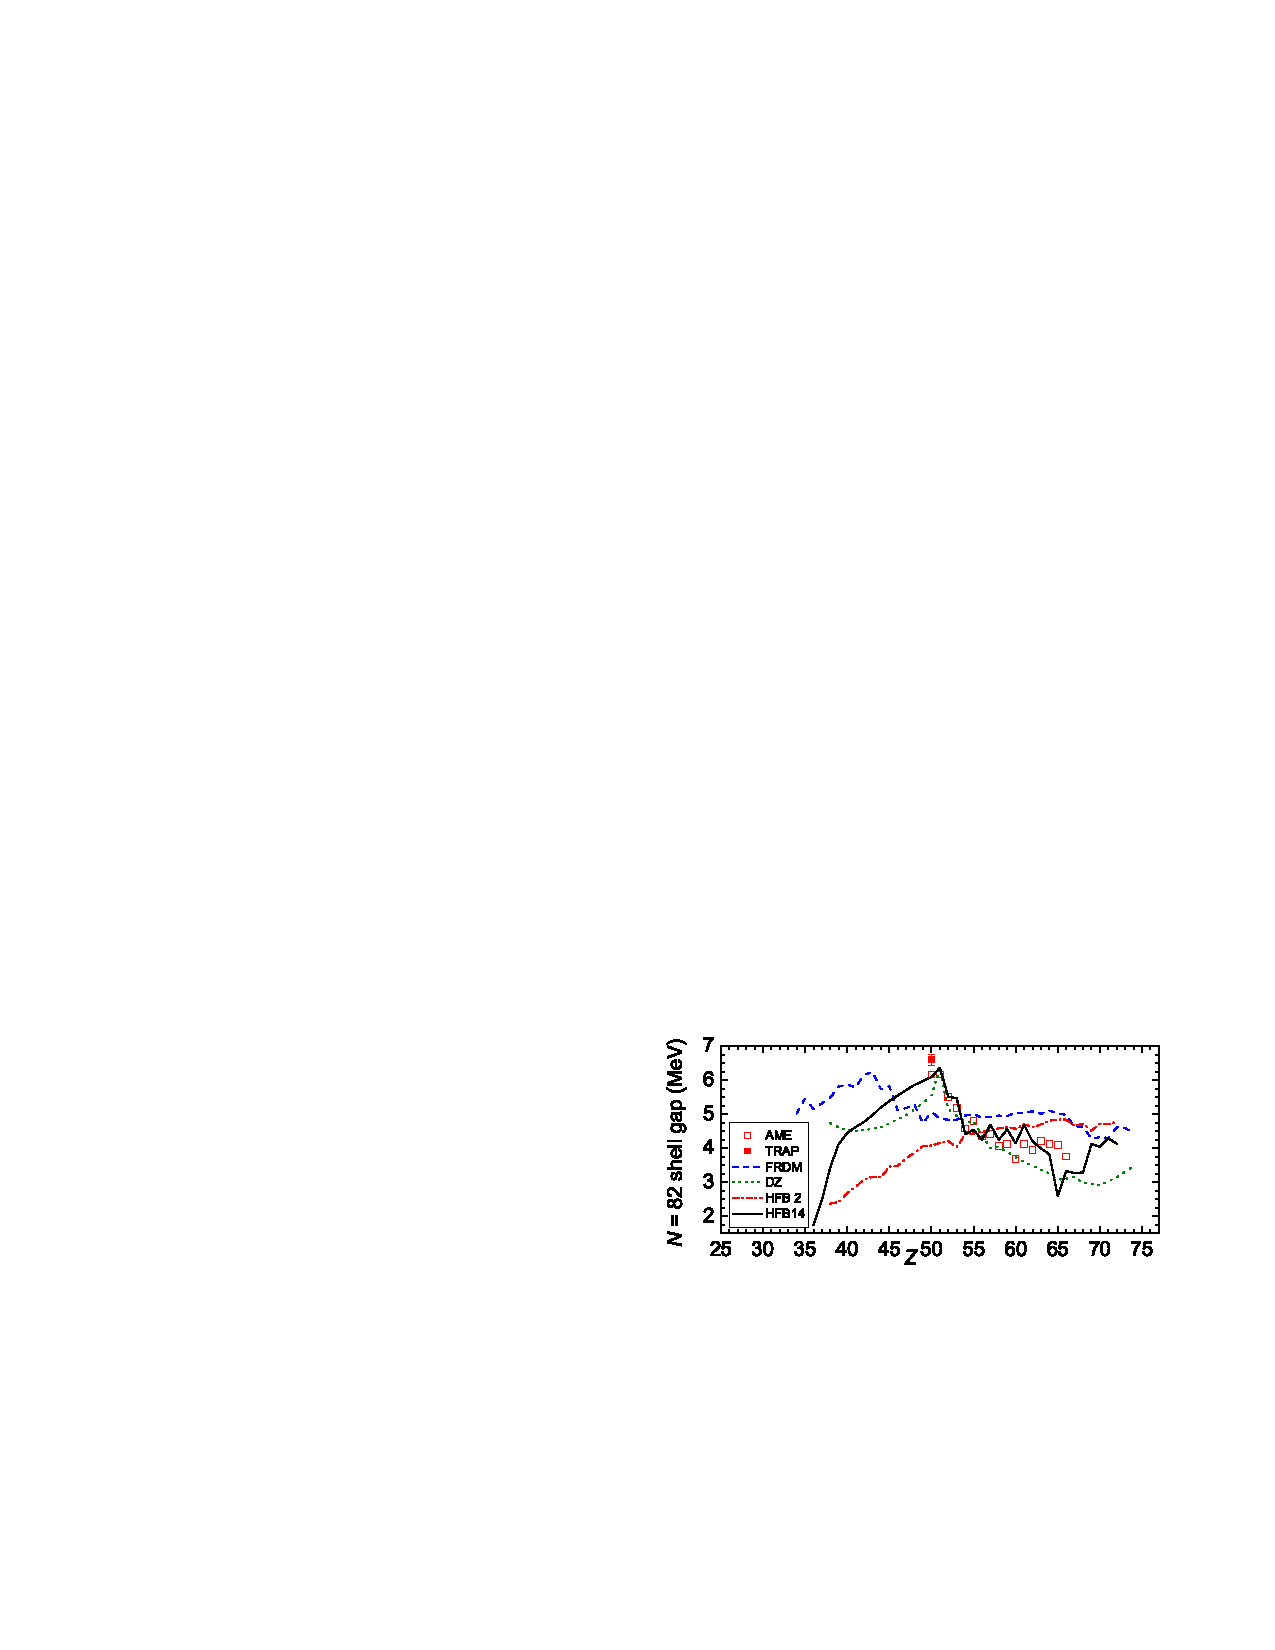
\includegraphics[width=0.75\columnwidth,keepaspectratio]{Dworschak_2008-fig3}%
\caption[Plot of the $N=82$ shell gaps as a function of $Z$]{Plot of the $N=82$ shell gaps as a function of $Z$.  The shell gaps are defined by the $S_{2n}$ energy and are determined experimentally from mass measurements.  Also plotted are a number of theoretical calculations.  The mass measurements show a peak at $Z=50$, corresponding to the doubly-magic nucleus $^{132}$Sn, meaning that the $N=82$ shell is not quenched in the tin isotopes.  Figure from Ref.~\cite[Fig.~3]{Dworschak_2008}.}%
\label{50_gap}%
\end{figure}

\subsection{Outlook}
In order to further the understanding of the $r$-process and the evolution of nuclear structure towards the neutron drip line, additional experimental data are required.  Even though $^{132}$Sn may appear to be less ``exotic'' than previously believed, its role as a doubly-magic nucleus along the $r$-process path cannot be overlooked or understated.  Information about the single-neutron states above the $^{132}$Sn shell closure will be vital to forming a complete picture of nuclear structure in this region.

At present, the majority of published experimental data related to energy levels of nuclei in the vicinity of $^{132}$Sn come from $\beta$-decay studies.  The first study of the single-neutron states in $^{132}$Sn was performed at ISOLDE~\cite{Hoff_1996}.  Indium isotopes were produced in by beam-induced fission of uranium and the subsequent $\beta$-decays were studied.  By measuring $\gamma$-rays in coincidence with the $\beta$-decays, the energy levels of the resultant $^{133}$Sn isomers were deduced.  Of the three energy levels proposed in this study, one has since been confirmed by measuring the prompt $\beta$-decay spectra following the spontaneous fission of $^{248}$Cm~\cite{Urban_1999}.  By gating on known isomeric transitions in $^{112}$Pd, a fission partner of $^{133}$Sn, the 1561\,keV transition, corresponding to the $h_{9/2}$ neutron level, has been confirmed.

Spins and parities can be tentatively assigned using $\beta$-decay selection rules and comparison to theoretical models, but no conclusive assignments can be made.  An additional problem with the $\beta$-decay studies in the $^{132}$Sn region is that they generally populate high-energy excited states~\cite{Hoff_1996}. The neutron separation energy of $^{133}$Sn is only 2.45\,MeV, so the higher energy states preferentially populated by $\beta$-decay are unbound against neutron emission, making them difficult to detect.   In order to effectively study the structure of low lying states it is necessary to use another method of measurement.  Direct nuclear reactions involving nucleon transfer provide a unique window to measure these quantities.  The $^{132}$Sn($d$,$p$) measurement performed by \citet{Jones_2010} is an example of such a reaction study; this measurement is discussed in Chapt.~\ref{standards}.